\ifdefined\XeTeXrevision\else\pdfoutput=1\fi
\documentclass[11pt]{article}
\usepackage[margin=1in]{geometry}
\usepackage{booktabs}
\usepackage{amsmath}
\usepackage{graphicx}
\usepackage{xcolor}
\usepackage{hyperref}
\usepackage{microtype}
\hypersetup{colorlinks=true, linkcolor=blue!60!black, citecolor=blue!60!black,
  urlcolor=blue!60!black, pdftitle={The Writer Wins, the Emitter Learns},
  pdfauthor={Franci Penov}}
\title{The Writer Wins, the Emitter Learns:\\Same-Day Answers to the Open Questions\\of the Composition and Cadence Notes}
\author{Franci Penov \\ kortexa.ai \\ \texttt{francip@kortexa.ai}}
\date{2026-08-09}

\begin{document}
\maketitle

\begin{abstract}
The composition note~\cite{penov2026thirdblock} and the cadence
note~\cite{penov2026carrier} each ended by naming its own missing
experiment: M3, the registered depth-partition control that would
separate ``one writer'' from ``writers that merely stopped colliding in
parameters,'' and C2b, the registered re-encoding consistency emitter
aimed at the cadence loop's one located failure. This note reports both,
run the same day, each landing on the side its parent note predicted.
M3: the creature pair's two blocks, retrained as independent single-lane
bridges on disjoint halves of the 4B host's eight full-attention layers
(393,216 parameters each, zero overlap, disjointness verified by
identity against the armed tower), are perfect solo
(1.00 at every seed) --- and every merged cell
sits at the floor: joint 0.000 at all three seeds, against the
one-writer bridge's 1.00/0.90/1.00 on the same items, with the
wreckage a different dominance pattern each seed. Composition dies in
the shared residual stream, not in parameter collisions; the one-writer
attribution stands. C2b: one consistency term --- the packet encoded
from a goal's canonical acted pass must reproduce the packet encoded
from its assignment exchange --- and the C1 gate still passes at every
seed (0.90/0.80/1.00 against 0.20 floors) while the re-run C2 loop
returns reading (i) unanimously: live re-emitted goal-consistency over
hops 4--7 rises from 0.20 flat to 0.80/0.60/1.00, matching each
seed's own frozen arm, one seed perfect across all sixteen ticks with
zero contamination. The mechanism the program was building toward is
now measured end to end at creature scale: one writer speaks for many
sensors, and a goal the model writes itself survives its own cadence.
\end{abstract}

\section{Two notes, two named gaps}

Paper 11 established that a single hypernetwork bridge reading $N$
sensors composes where every merged-writer route had died, but declined
to attribute the win between ``one writer'' and ``natively-trained
joint data'' --- M3, registered beside M1, was named as the experiment
that separates them. Paper 12 established that a goal packet endures
sixteen ticks when replayed frozen but dies on its first re-encoding,
located the failure in the emitter's training distribution, and named
C2b --- registered before anything ran --- as the follow-up. Both
experiments ran on 2026-08-09, the day their parent notes were
published. This note is the pair of answers.

\section{M3: writers that cannot collide still fail}

The design removes parameter interaction entirely. The
\texttt{temporal$+$vitals} blocks were retrained from scratch
as independent single-lane bridges --- the M1 recipe, one lane each, no
joint data --- with LoRA targets on disjoint halves of the eight
full-attention layers: lane A on layers
3, 7, 11, 15, lane B on layers
19, 23, 27, 31, 393,216
parameters per half, tiling the original channel exactly. Merging is
concatenation: each block owns its layers outright, and the harness
verifies the disjointness by identity against the armed tower rather
than assuming it from a path convention.

\begin{table}[t]
\centering
\small
\setlength{\tabcolsep}{5pt}
\begin{tabular}{lrrrrrrr}
\toprule
seed & solo A & solo B & merge joint & merge A/B & shuffled & M1 joint & fit A/B \\
\midrule
42 & 1.00 & 1.00 & 0.000 & 0.20/0.30 & 0.000 & 1.00 & 0.86/0.95 \\
1042 & 1.00 & 1.00 & 0.000 & 0.40/0.10 & 0.000 & 0.90 & 0.89/0.96 \\
2042 & 1.00 & 1.00 & 0.000 & 0.10/0.70 & 0.000 & 1.00 & 0.90/0.96 \\
\bottomrule
\end{tabular}
\caption{M3 at 4B, \texttt{temporal$+$vitals}: depth-partitioned
independent writers, merged by concatenation. Every seed is valid (solo
retention perfect) and every merge sits at the floor the one-writer
bridge cleared on the same items.}
\label{tab:m3}
\end{table}

The result (Table~\ref{tab:m3}, Figure~\ref{fig:followups} left) is
unambiguous. Solo, both halves are perfect: 1.00 A-heed and
1.00 B-heed at every seed --- a half-depth channel loses
nothing on its own lane. Merged, joint-heed is \textbf{0.000 at every
seed}, and the per-lane rates collapse to a dominance pattern with a
different winner each seed
(0.20/0.30; 0.40/0.10; 0.10/0.70)
--- both lanes degrade, neither survives whole, the joint never fires.
The state-deranged shuffled merge sits at 0.000, and the router-oracle
on the retrained solos is 0.000 --- selection still cannot make one
utterance satisfy two scorers. This is paper 7's layer-partition lesson
reproduced at the M1 venue with the M1 recipe: zero weight-space
interference buys nothing, because composition dies in the shared
residual stream --- there is one stage no matter how the writers are
wired. \textbf{The attribution closes: M1's win is the natively-trained
single writer.}

\section{C2b: one consistency term closes the emitter}

C2's diagnosis was exact: the emitter (the layer-12 tap plus the
bridge's encoder) was trained only on assignment-exchange surfaces, and
the loop hands it \emph{acted} passes --- the serve-time action menu
plus a JSON tool call --- which it encodes off-distribution, losing the
goal in one hop. C2b, registered before anything ran, adds exactly what
the diagnosis asks: for each training item with goal $G$, the canonical
acted surface under $G$ is also encoded, and the training gains
$1-\cos(\mathrm{enc}(\text{acted-}G),\,
\mathrm{sg}[\mathrm{enc}(\text{assignment-}G)])$ plus the
auxiliary goal classifier applied to the acted packet --- the
assignment side stop-gradiented so the original regime stays the
anchor. Everything else is C1-verbatim, and the protocol re-checks the
C1 gate before any loop runs: the consistency term must not buy loop
stability with C1's currency.

\begin{table}[t]
\centering
\small
\setlength{\tabcolsep}{5pt}
\begin{tabular}{lrrrrrrr}
\toprule
& & \multicolumn{2}{c}{live 4--7} & & & \\
\cmidrule(lr){3-4}
seed & C1 gate & C2 & C2b & live 0--3 & post-switch & frozen 4--15 & contam. \\
\midrule
42 & 0.90 & 0.20 & 0.85 & 0.80 & 0.80 & 1.00 & 8/40 \\
1042 & 0.80 & 0.20 & 0.60 & 0.60 & 0.65 & 0.60 & 7/40 \\
2042 & 1.00 & 0.20 & 1.00 & 1.00 & 1.00 & 1.00 & 0/40 \\
\bottomrule
\end{tabular}
\caption{C2b at 230M: the C1 gate re-check and the re-run C2 loop. The
live 4--7 column pairs each seed's C2 baseline with its C2b value; the
frozen column is the carrier ceiling the live arm now matches.}
\label{tab:c2b}
\end{table}

It does not (Table~\ref{tab:c2b}): goal-consistent choice on held-out
phrasings is 0.90/0.80/1.00 against the same three floors C1
measured (no packet 0.20, undirected waking 0.20, wrong-goal packet
above both), zero-dose bit-exact, base weights byte-identical. And the
loop, re-run verbatim, returns \textbf{reading (i) at every seed}
(Figure~\ref{fig:followups} right): the live re-emitted arm holds at
0.80/0.60/1.00 over hops 4--7 where the C2 emitter sat at 0.20
flat, the hop-1 collapse is gone, and at every seed the live arm now
matches its own frozen arm --- seed 2042 runs all sixteen ticks at
1.00 with zero contamination, and seed 1042's weaker 0.60 is exactly
its frozen ceiling, so the re-encoding itself now costs nothing.
Post-switch consistency is 0.80/0.65/1.00 with contamination
0--8 of 40. The registered
caveat travels with the result: the canonical acted surface covers
goal-consistent replies, so off-policy passes --- a tick that acts
wrong or emits malformed JSON --- remain the named residual, and the
on-policy question belongs to the tool-pursuit line.

\begin{figure}[t]
\centering
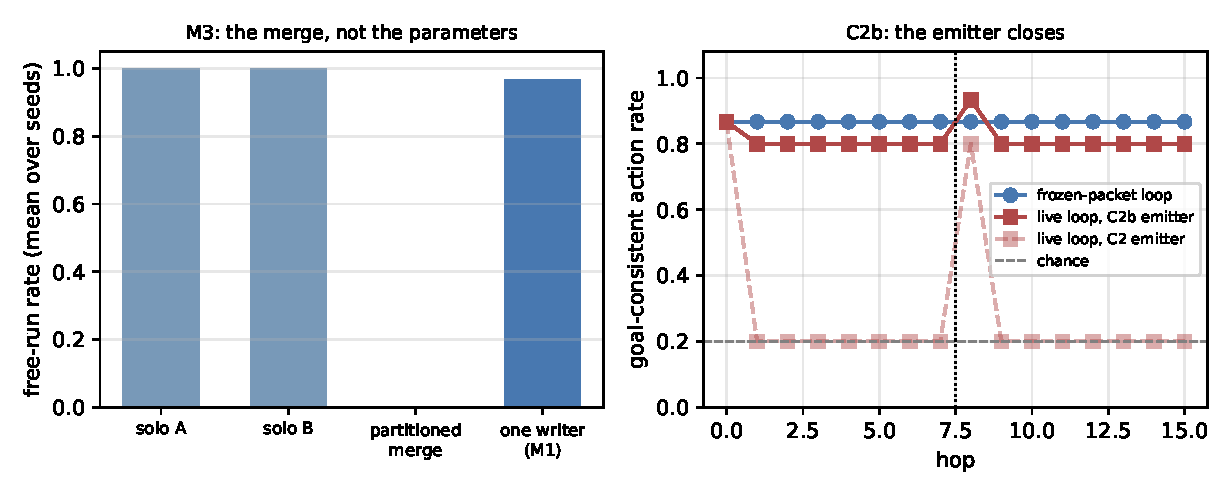
\includegraphics[width=\linewidth]{followups.pdf}
\caption{The two answers. Left: M3 at 4B --- depth-partitioned writers
are perfect solo and dead merged, while the one-writer bridge composes
on the same items. Right: C2b at 230M, pooled over five goals and three
seeds --- the same sixteen-tick loop that collapsed at hop 1 under the
C2 emitter (faded) holds at the frozen arm's level under the
consistency-trained emitter; the dotted line marks the scripted goal
switch.}
\label{fig:followups}
\end{figure}

\section{What stands now}

The two parent notes' claims compose. Multi-sensor conditioning of a
frozen host is solved by one trained mouth-piece, and M3 shows the
mouth-piece --- not the absence of parameter collisions --- is what
does the work. A goal in 256 floats directs action, survives frozen
replay indefinitely, and now survives its own re-encoding: the
creature-scale loop --- write the want, act under it, re-write it from
the acted pass, tick after tick, with a clean scripted switch --- is
measured working end to end. What was a research gap this morning is a
deployment decision tonight, and that decision is held for a human by
standing rule. The open edges are the registered ones: on-policy acted
surfaces, $N$ beyond three, and the inserted-capacity control (M2).

\section{Reproducibility}

Artifacts \texttt{multi-sensor-m3-4b} and
\texttt{own-cadence-c2\{,b\}-230m} are bundled beside this note;
every number and the figure render from them alone. Harnesses:
\texttt{multi\_sensor.py --stage m3} and
\texttt{own\_cadence.py --stage c2b}, in
\texttt{tracks/multi-sensor/} and \texttt{tracks/own-cadence/};
registrations and results, each dated before its run, in the tracks'
\texttt{PLAN.md} files. Hosts: frozen
Qwen3.5-4B (M3, CUDA) and frozen LFM2.5-230M (C2b, MPS float32).

\begin{thebibliography}{9}
\bibitem{penov2026thirdblock} F.~Penov. The Third Block Composes:
One-Writer Bridges for Multi-Sensor Conditioning of a Frozen Language
Model. Preprint, 2026.
\url{https://github.com/kortexa-ai/legolm.basis}.
\bibitem{penov2026carrier} F.~Penov. The Carrier Holds, the Emitter
Leaks: A Goal Packet on Its Own Cadence at Creature Scale. Preprint,
2026. \url{https://github.com/kortexa-ai/legolm.basis}.
\bibitem{penov2026interference} F.~Penov. Zero Weight-Space
Interference Is Not Enough. Preprint, 2026.
\url{https://github.com/kortexa-ai/legolm.basis}.
\bibitem{penov2026onemouth} F.~Penov. One Mouth, One Mode. Preprint,
2026. \url{https://github.com/kortexa-ai/legolm.basis}.
\end{thebibliography}

\end{document}
